\documentclass[5p,twocolumn,final]{elsarticle}


\makeatletter
\def\ps@pprintTitle{%
 \let\@oddhead\@empty
 \let\@evenhead\@empty
 %\def\@oddfoot{\emph{Essay for ``Information Governance'', TU Berlin   \hfill Submitted: \today}}%
 \let\@evenfoot\@oddfoot}
\makeatother


\usepackage{appendix}
\usepackage{lipsum}
\usepackage{lineno,hyperref}
\usepackage[dvipsnames]{xcolor}
\usepackage{lettrine}
\modulolinenumbers[1]
\usepackage{natbib}
\usepackage{relsize}
\usepackage{comment}
\usepackage{setspace}

\hypersetup{
    colorlinks=true,
    linkcolor=blue,
    urlcolor=blue,
    citecolor=blue
}
\usepackage{titlesec}
\titlelabel{\thetitle\quad}
\titleformat{\section}{\Large\bfseries}{\thesection}{1em}{}


\begin{document}
\begin{frontmatter}
	\title{\LARGE\textbf{Is the Search Engine Market still open to new players? You.com as a Case-Study }}
\author{Clemens Frey (457127), Elias Safo (458423), Jannik Novak (392210), Joy Lucas (456583)}
\begin{keyword}
    Search Engine, You.com,  Network Effects, Transaction Costs, Competition, Privacy
\end{keyword}

\end{frontmatter}

%\linenumbers
\pagenumbering{arabic}


\section{Abstract} The search engine market is predominantly controlled by a small number of private companies. As a consequence, startups trying to succeed face enormous challenges. This paper introduces these challenges and discusses specific strategies You.com - a search engine startup - uses to establish itself on the market. The most significant being the combination of AI implementations, privacy, and search. We investigate whether this unique search experience has the potential to attract a large user base. Lastly, we propose ways for You.com to become profitable and establish a firm presence in the market.

\section{Introduction}
%\lettrine[lines=2]{\textbf{Y}}
 You.com was founded by Bryan McCann and Richard Socher on November 9th, 2021. There are various functionalities offered on You.com that are meant to differentiate it from other search engines. The founders of You.com have repeatedly emphasized their focus on privacy, while still leaving the user options for a personalized experience. To achieve this, You.com offers users two modes of interacting with the search engine.  In private mode, no personal data is collected~\cite{youcom}, here, personal data refers to the information of an identifiable natural person as defined in Article 4(1) of the GDPR. In personal mode, a minimal amount of personal data is collected. You.com also gives users the ability to customize their search experience by upvoting sources they find relevant and downvoting sources they find less helpful. Upvoted sources will be shown more frequently and downvoted sources will be lower in the search results. In addition to that, You.com offers various AI tools.
\begin{itemize}
    \item With YouWrite, users choose a topic and an AI generates a text related to the chosen topic.
    \item With YouChat, users can ask questions and have a conversation.
    \item With YouImagine, users describe an image and are presented with an image fitting the description.
    \item With YouCode, users can describe a problem, stating a preferred programming language and an AI will generate code to solve the problem.
\end{itemize}
Being a startup company that has entered the search engine market only recently, it can be said that You.com is still in the early stages of establishing itself.
For any search engine company to achieve a firm market position, there are hurdles it must overcome in building a wide user base and assuring the longevity of its product. In the following we analyze part of these challenges, considering reports of search engine companies that have started in a similar position. \par
Our essay will be structured as follows: In Section 3 we introduce the various challenges that aspiring search engine companies are presented with when entering the market. In Section 4 we examine the strategies employed by You.com to create a viable monetization path. Section 5 discusses the strategies used to ignite network effects and reduce transaction costs. In Section 6 we investigate You.com's privacy policy and compare it to the policies of other search engine providers like Google. To this effect, we will also consider its underlying problems. Finally, Section 7 concludes our findings with an evaluation of the search engine and its chances for future success.
%
\section{Competing in the search engine market}
According to the reports of search engine providers like DuckDuckGo and Ecosia, there are many similar challenges, businesses encounter when trying to establish themselves in the search engine market. Many of these challenges arise from having to compete with the well-established Google and Microsoft.~\cite{green_business, duckduckgo_whitepaper} \par
While You.com offers a product that can be regarded as competitive, in the sense that it provides a lot of the functionalities that end users expect from a search engine nowadays - and more, the question can be raised, whether offering a competitive product is enough to be successful. \par
A challenge for aspiring search engine companies lies in the acquisition of a wide range of up-to-date web links. This requires the use of so-called web crawlers - tools that are used to scan the internet for web pages, which many websites block unless they are from Google and Microsoft. For this reason, Google and Microsoft are the only ones currently providing a significantly large and updated web-index.~\cite{duckduckgo_whitepaper} \par
Another challenge lies in collecting large amounts of data in the form of user searches, which could then be used to improve search result rankings by providing more relevant results for specific search queries.~\cite{google_data} This is an issue that is less relevant for You.com since their product focuses on providing personalized search result rankings through the use of machine learning algorithms. Search result rankings are therefore improved over time using data provided by the individual user.~The collection of data among all users of You.com is less required.~\cite{youcom_ai} \par 
On the contrary, the obstacle of acquiring a sufficiently large amount of organic web links, is more significant for You.com. Like most smaller search engine companies, You.com thought it necessary to sign a search syndication contract with either Google or Microsoft. Having signed such a contract, they are allowed to display some of the organic web links provided by Microsoft, in their own search results. A search syndication contract comes with the condition, that the purchasing party shows advertisements next to the organic web links that they have acquired. The advertising revenue is then split up between the two parties.~\cite{duckduckgo_whitepaper} \par
Since the acquisition of organic web links comes with not insignificant costs, aspiring search engine companies need a means of monetization. Most achieve this with advertising, which will lead them to Google and Microsoft, the only providers of a large-scale search ad infrastructure. Search engines trying to rely only on independent advertisers, such as for example Amazon, will likely not generate sufficient revenue to make up for the costs of purchasing organic weblinks.~\cite{duckduckgo_whitepaper} We will discuss You.com's monetization strategies in more detail in the next section.\par
Search ads, in particular, benefit from network effects due to their auction-based sales principle. This means, that an advertisement related to a specific keyword, like for example "headphones", will sell for a higher price when more advertisers are bidding on that keyword. Many previous search ad providers combined, in order to benefit from these network effects, leaving only Google and Microsoft.~\cite{duckduckgo_whitepaper} \par


\section{Monetization}
In three rounds of funding, You.com has managed to accumulate \$45M.~\cite{crunchbase} To ensure the longevity of the company, it will have to become self-sustainable, in other words, they have to generate a sufficient amount of profit to compete in the search engine market.
To this end, the company requires ways of monetizing its product.\par
As of February 2023 there are only two ways You.com generates any revenue. Firstly, the company provides a subscription model for some of its AI tools, including YouWrite. After a free trial period, users can choose between two subscription models. This use of versioning allows You.com to provide different features based on their customer's willingness to pay.~\cite{linde2009pricing}
Secondly, You.com earns a percentage of products sold through affiliate links on certain apps, e.g., the Walmart-app.~\cite{youcom_ai}\par
A major strategy for search engine providers to generate revenue lies in the use of ads. For now, You.com focuses on user growth and does not show any ads. The company has already announced, that this will most likely change in the near future.~\cite{youcom_ai} However, according to the company, ads will be private or non-personalized, meaning, that personal interests tied to a specific user won't be tracked for the purpose of running targeted ads.~\cite{farahat2012} Instead, You.com plans on implementing keyword-based private ads. Ads will be shown according to their relevance for specific search queries. For instance, a search query containing the keyword "cars", will be accompanied by ads from automobile companies. \par
There are currently other competitive search engine companies that have successfully become profitable using similar strategies. For example, DuckDuckGo has become a real competitor in the search engine market in Europe and North America, using only affiliate links and private ads.~\cite{thinkinsights} \par
The key motivation for rejecting personalized ads for You.com as a company comes from the fact that You.com heavily advertises itself as a "Private Search Engine". To this effect, the search engine makes a lot of claims in regard to their privacy policy and has implemented a "Private" mode.
Privacy has been proven to be a competitive differentiator in search engines. Companies like DuckDuckGo have successfully acquired a substantial user base, using privacy as a distinguishing feature to differentiate themselves from competitors.\par
It is important to keep in mind that many early-stage platforms utilize phrases such as "privacy" or "AI" as buzzwords, mainly to attract users. To identify whether You.com aims its focus at keeping its user's data private, it is imperative to take a closer look at its privacy policy.

%\lipsum[1]

\section{Network effects and transaction costs}

\subsection{Network effects}
% concrete problem
For this and many other start-ups user growth is front and centre in almost everything they do.
%sbstract problem
The main challenge is to reach a critical mass \cite[p.15 ff.]{shapiro1999} i.e. a user base large enough that it continues to grow organically without the necessity of interference by the company.\\
One possible driver for user growth is a positive feedback loop \cite[p.175 ff.]{shapiro1999}, where more users add more value to a platform e.g. eBay or Facebook. Looking at search engines, it is not so clear if the concept of a feedback loop is applicable since search engines are not social platforms, meaning that a single user is not affected by how many others are using the search engine \cite{varian2017}. Therefore direct network effects are much harder to achieve. \par
According to Varian \cite{varian2017}, \textit{"Network effects are a demand-side phenomenon (value depends on share) […] firms with different cost functions of production for quantity or quality can easily co-exist"}. Here production quality refers to the fact that different companies can develop algorithms that address different needs of different users independently of the market share of other larger companies. We are now examining how You.com achieves just that.\par
%Advertisment revenue: Mehr User führen zu mehr Advertisern, aber mehr Advertiser führen kaum zu mehr Usern, das Gegenteil ist wohl eher Fall. Wir müssen also andere Faktoren betrachten, die den User Growth treiben.%
You.com is planning on developing its Apps such as News or Snippet "in-house" to ignite the positive feedback loop \cite{techcrunch2022}. More of these apps should then lead to more users which find them useful, which in turn brings more external developers to the platform that builds such apps. Those apps attract even more users and we have a positive feedback loop.

\subsection{A Multi-Sided Platform}
You.com is trying to acquire two main user bases. One of which is the consumers, using You.com as a service. The other is developers, writing code for new apps and features. 
Each group of users affects the other, in that a small user base reduces the incentive to write apps for you.com and a small number of apps, features, and tools reduces the incentive to use You.com. As such, you.com shows the features of a MSP ( multi-sided platform). \par
%
The "Chicken-and-Egg dilemma" \cite{caillaud2003}, the problem of the demand side of a platform being influenced by the supply side and vice-versa is one seen quite commonly in early-stage MSPs.
There exists a need for a critical mass of suppliers to attract enough demand for a platform. However, if there is little demand for a platform, the supply side is unlikely to adopt the platform.
As soon as the critical mass for all user groups of the MSP is reached, this effect can stimulate platform growth.\par
%
There are a few strategies that can help overcome the "Chicken-and-Egg dilemma" for early-stage MSPs, some of which You.com has already implemented or may implement in the future. 
One of the Strategies to overcome this "Chicken-and-Egg dilemma" is to focus the resources of a platform on a particular target group first. Once the critical mass is reached in a single group, an MSP may expand to a broader target group.\cite[Section 2.1]{linde2009pricing}\par 
%
For search engines, this means focusing on a single niche of users to begin with. In the case of You.com, this niche consists mainly of tech-averse users. This becomes apparent looking at AI tools such as YouCode and YouChat.\par
%
Another strategy for overcoming the "Chicken-and-Egg dilemma" for early-stage MSPs is platform staging. This entails developing one side of an MSP to build an incentive for the other side to join.\cite[Section 2.2]{linde2009pricing}\par
%
In the case of you.com, this strategy was applied to the production of their apps. In the long run the search engine plans on outsourcing the majority of its app development. In order to incentivize developers to adopt the search engine's platform, you.com has developed the first 200 apps themselves.~\cite{techcrunch2022}
%
This is meant to attract a subset of eventual users which in turn incentivizes developers to write apps for the platform.\par
Side Switching is another strategy for overcoming the "Chicken-and-Egg dilemma" for early-stage MSPs. The concept of side switching is to try and turn a multi-sided platform into a one-sided platform by allowing users to fill either market side of the MSP. Typically this requires either side of the MSP to be as simple as possible, to allow users to switch freely between sides.\cite[Section 2.6]{linde2009pricing}\par
%
In the case of You.com the developer side of the platform requires a lot more knowledge and skills than the consumer side. However since the target audience of the platform mainly consists of tech-savvy users, You.com may be able to get users to help in the development of the platform.

%%%

\subsection{Transaction costs}
Having looked at how You.com attracts users to their platform, we will now look at how You.com reduces transaction costs to keep those users on the platform.\par
% Concrete problem
Different situations require different needs. Those may be: having to write an essay about data protection, which entails reading several papers, skimming websites, or searching for information in a book. But there are instances where a User is not interested in details but rather wants a quick and concrete answer or solution to his question. For example, a user may want to write a syntactically correct python function that multiplies two matrices without having to read the python documentation or without having to spend hours searching through online forums. Here the user encounters two main challenges: 1. finding the right sources of information and 2. comprehending the information. \par
% abstract problem
The interaction with a product of a company is referred to as a transaction~\cite{williamson1989}. Considering web search these transactions produce both, search costs and information costs, which the user of the said product has to bear.
Search costs refer to the time spent searching for a source of information~\cite[p.126]{shapiro1999} and information cost refers to the effort of extracting the - for the user relevant - knowledge from a source.\par
% abstract solution
The general strategy is to lower those transaction costs, i.e. improve the quality of service for the end user. This can surely be achieved through engineering solutions, if we look at any industry, the companies with the most resources usually can afford to employ the best engineers. Those then build the best software/ devices which in theory have minimal transaction costs. But that alone can't guarantee success, if it could companies like Instagram wouldn't exist since Facebook had industry-leading engineers when Instagram emerged as a startup. Especially in the case of tech companies are UI Design decisions crucial for a successful product that minimizes transaction costs. \par
% concrete solution: design decisions --> You.Chat window and parallel view; engeneering methods --> AI,etc.
You.com applies both engineering methods and design decisions which aim at minimizing transaction costs. An already established UI method is Google's Answer Box~\cite{miklovsik2016}, which provides the user with a short answer to a search query without the need of opening any website. You.com developed this method significantly further in two ways. \par Firstly, its horizontal alignment of search results [Figure 1] makes it easier to access multiple web pages at once. Given a sufficient page rank algorithm~\cite{duhan2009IN} it is most likely that a user who searches for matrix multiplication finds a suitable web page from the 1st to let's say the 6th result. In the worst case, a user would need to skim through all 6 pages until he finds the right one. And precisely because You.com aligns those 3-6 first web pages horizontally for the user to look at, the search costs are lowered significantly. \par
Secondly, You.com combines its search engine with the AI chatbot YouChat. This chatbot generates an explanation or elaboration for whatever the search query was.  What this achieves is that the user understands the information seen on the search result without having to read the actual text on the website. In the previous example, this means YouChat explains to the user how matrix multiplication in numpy works, and this lowers the information cost. \par
Lastly, You.com addresses handling costs, which usually refers to the cost of finalizing a legal contract such as payments to a company or signing a lease contract. In our context handling costs refer to the time a user has to spend on selecting and copying a piece of code found on a website and pasting it inside his/her IDE. This cost gets significantly reduced through You.com's code snippet tool (as seen in Figure 1) which prepares a code from the search results on the left, to be copied by a single mouse click.
\begin{figure}[h]
\centering

\includegraphics[width=9cm]{numpy mult - You.com.png}
\caption{You.com Search query}
\label{fig:fig1}
\end{figure}

\section{Privacy}
The CEO of you.com Richard Sorcher has stated in multiple interviews that privacy is a priority for You.com~\cite{sorcher2022}. This has been one of their main strategies to get the upper hand over other Search engines like Google. With billions of searches per day Google is by far the most used search engine. Today it is involved in numerous antitrust cases over privacy concerns regarding e.g. unlawful processing of personal data~\cite{council_of_state}, and non-consensual sharing of user data with third parties~\cite{aepd}.\\
Leaving many users concerned about how their personal data may be violated. You.com addresses these concerns through privacy engineering.

\subsection{The Problem}
Google collects all types of data through their search engine. They collect two main types of data, data that users give to them such as names, passwords, phone numbers and payment information as well as data that is collected when their services are used such as device information, IP addresses, location and information about users activities like terms users search for, videos users watch, interactions with ads, voice and audio information, people with whom users communicate or share content, activities on third party sites, browsing history and purchase activity.~\cite{googleprivacy}
Data collection is considered harmful for multiple reasons. Some of the issues that arise from data tracking are the following.
\begin{itemize}
    
 \item{Data breaches:} With a vast amount of valuable user data being stored centrally on servers, the company could be subject to cyber-attacks. This trend has been seen across the tech industry like Yahoo(2013-2016), Microsoft(2021) and Facebook (2021). 
Data breaches can lead to identity theft, exposure of sensitive information and fraud~\cite{hammouchi2019}
\item{Manipulation:} Data collected can be used to manipulate people's decisions and behaviours without them even realizing, for example through targeted advertising.~\cite{thomas2018}
\item{Discrimination:} Data tracking can lead to bias or discrimination. For example, using targeted ads to advertise jobs or insurance to a certain race.
\end{itemize}

\subsection{What you.com claims to do differently}
Before looking into You.com's privacy policies it is important to understand the difference between personal and non-personal data. In the European data protection framework, personal data is data that directly or indirectly relates to an identified or identifiable natural person, while non-personal data refers to data that does not relate to an identified or identifiable natural person. To differentiate between personal and non-personal data, a legal test is used, which takes into account all means reasonably likely to be used to identify the natural person, such as the costs and time required for identification, as well as the available technology at the time of processing.~\cite{pallas2020}\par
%
You.com offers two modes personal mode and private mode.\\
 With Private mode you.com claims to not collect any personal data,  However, it should be noted that some non-personal data might still be collected for technical purposes or to improve the service. There are no cookies, no location data, and no search histories. This however comes at a cost, without collecting any data you.com cannot provide all their services. Features which require location are disabled for example “supermarkets near me” will not be able to provide users with supermarkets near them. Private mode users also miss out on the benefit of targeted ads.\par 
 %
 With personal mode, you get access to all features at the cost of sharing some data. They only collect the essentials and claim not to share it with 3rd parties without anonymizing the data. Some of the data they collect includes your name, password, and email (if you create an account), your app preference, your location, and your searches. Comparing the privacy policies of Google and you.com [Figure 2] the main difference is that you.com does not use your data for targeted ads.

%\autoref{fig:fig2}
\begin{figure}[h]
	\centering
    %\fbox{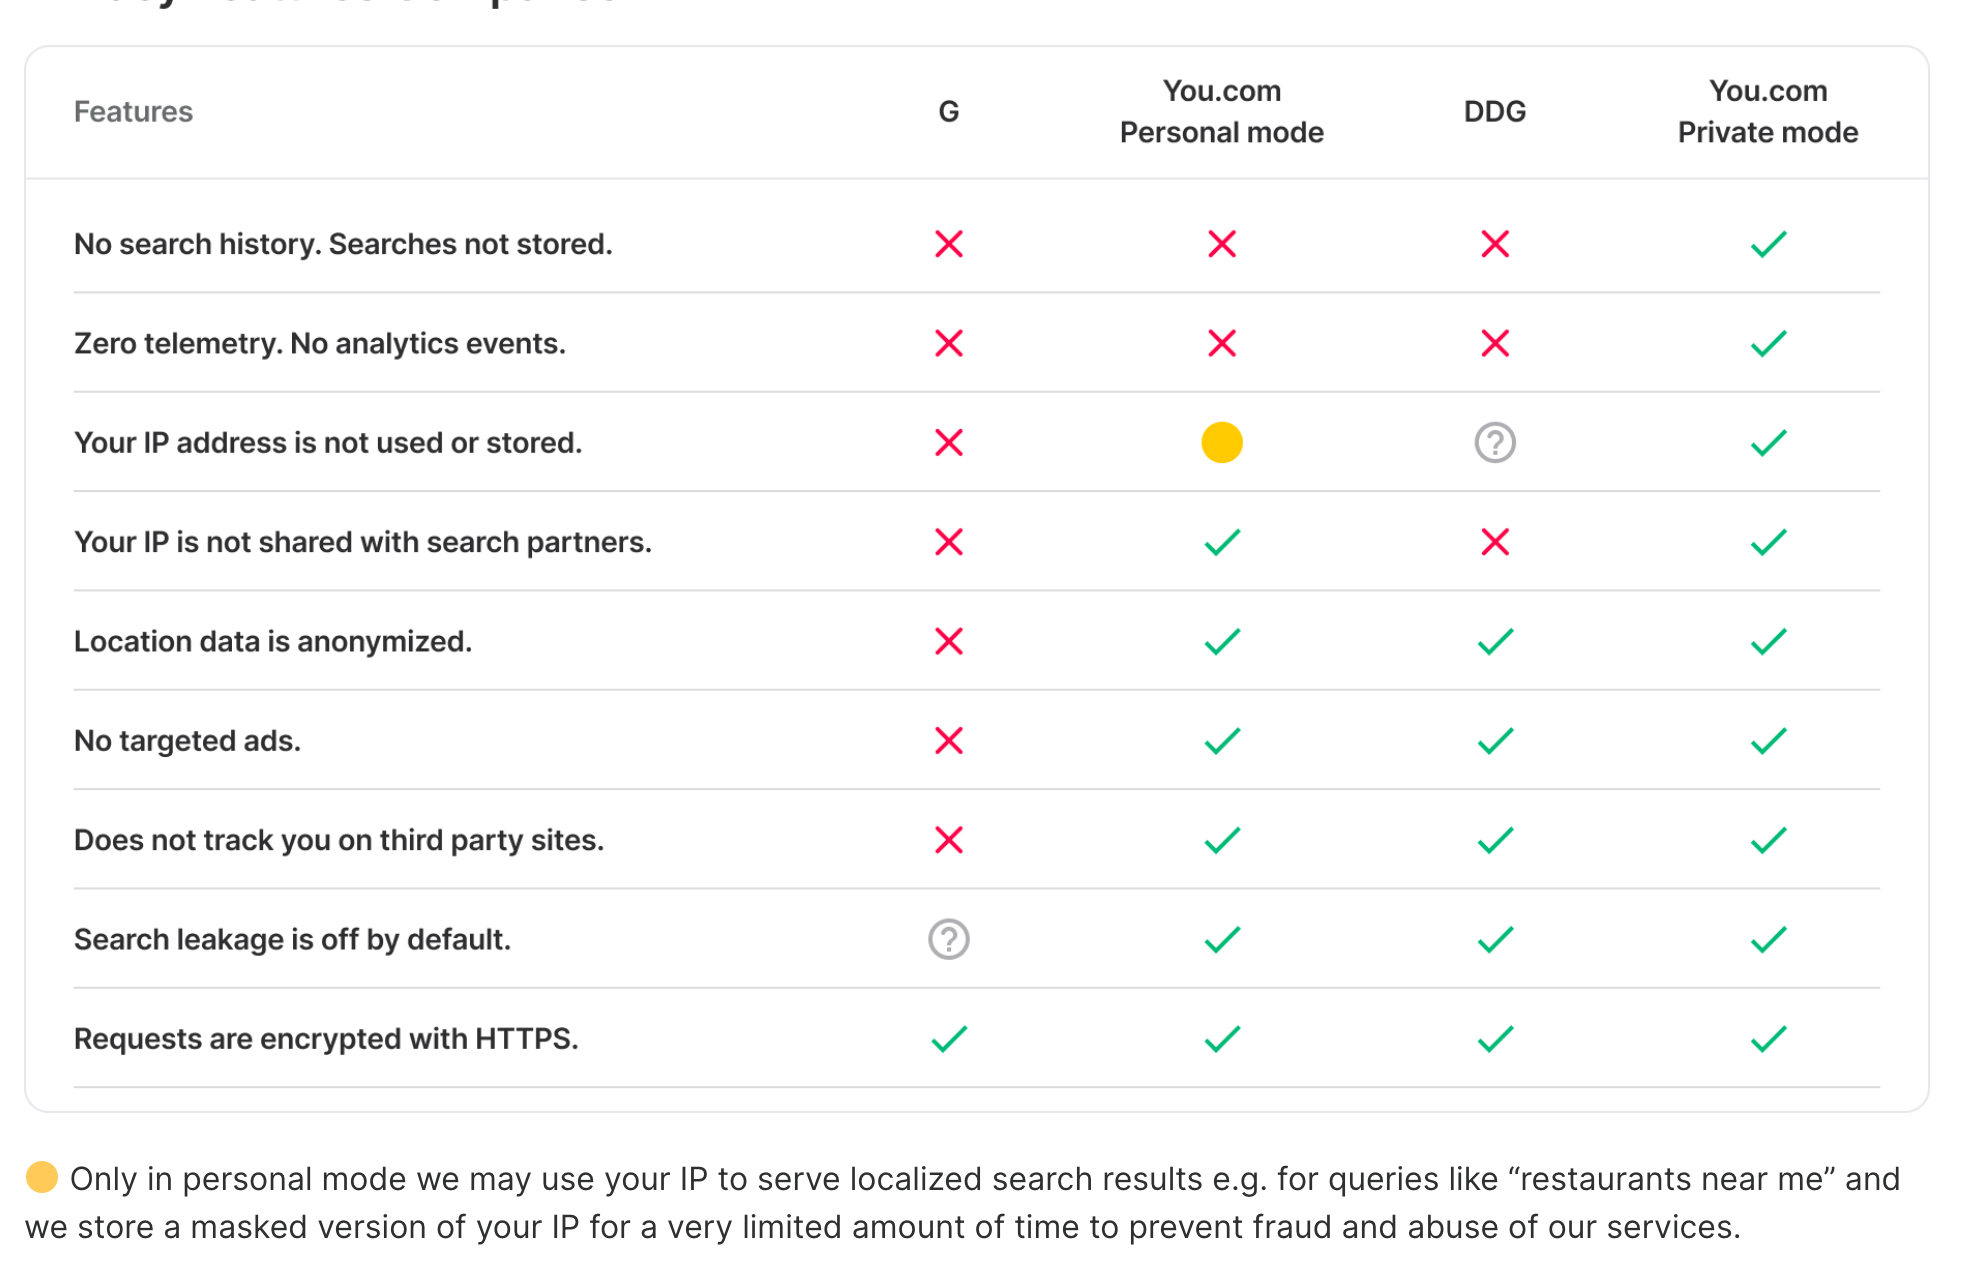
\includegraphics[width=9cm]{You.comVsGooglwe.png}} % Proxy
	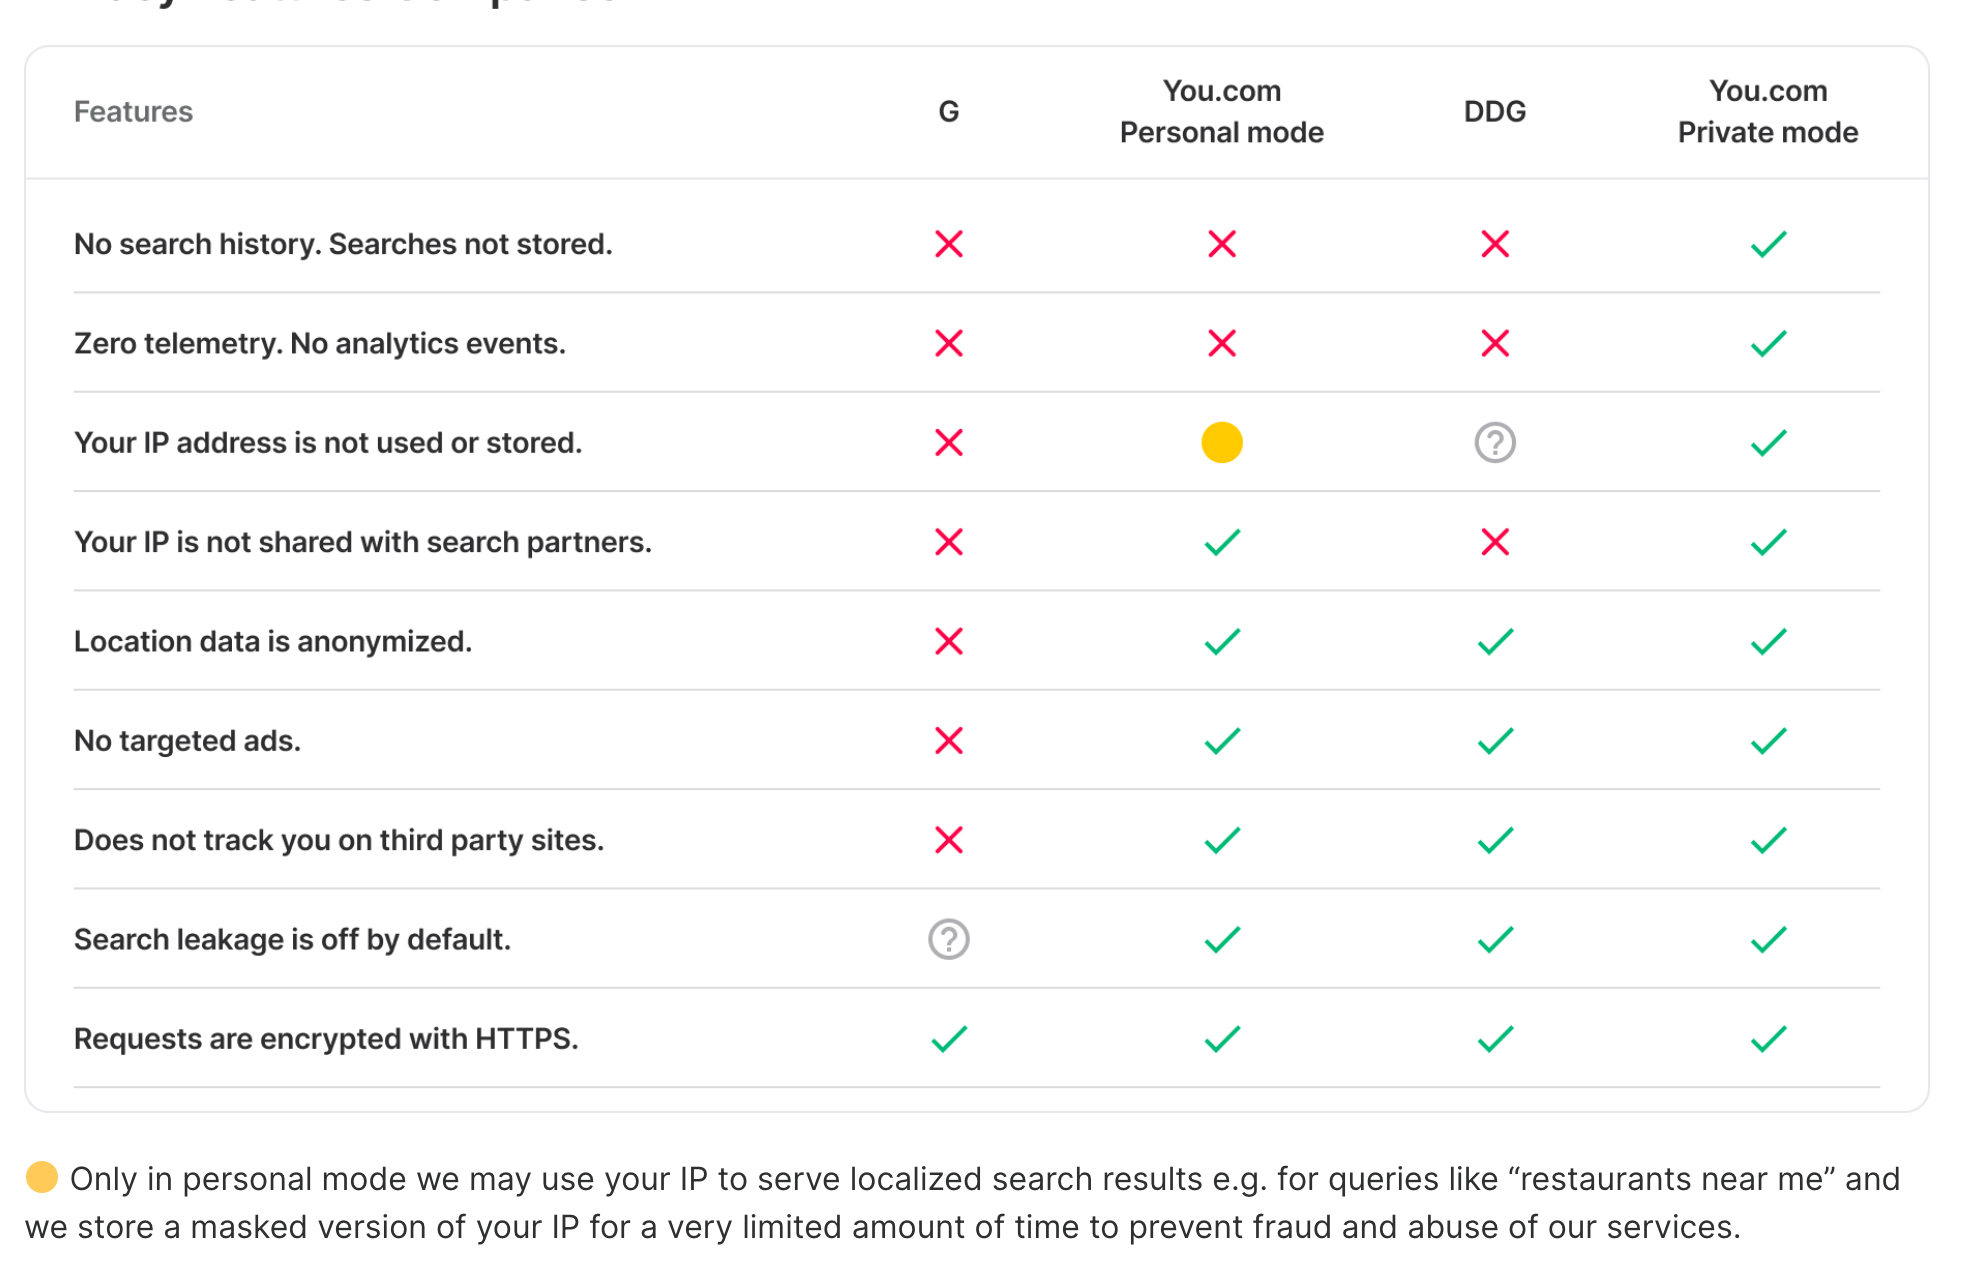
\includegraphics[width=9cm]{You.comVsGooglwe.png} % Proxy
	\caption{Search engine privacy comparison}
    \label{fig:fig2}
\end{figure}
\par 
You.com personal mode and Google differentiate in 4 rows. IP address sharing with 3rd parties and anonymization of search location are both claims google makes in its privacy policies. Whether search location can be considered as personal data depends on You.com's anonymization level. Giving you.com the upper hand only in non-targeted ads and no tracking on third-party sites.~\cite{youcom}\par
%
You.com’s privacy campaign is a classic example of non-price competition strategy. This can 
also be seen in apps like Signal Messenger. By emphasizing these features and building a reputation as a privacy-focused company, it is able to attract users who are concerned about data security and privacy.\par
%
You.com claims to offer a private search engine experience for its users. However, its privacy policies raise some concerns about user data collection and the lack of transparency in its data-sharing agreements.
 Moving forward, the company can improve its privacy policies by being more transparent about its data-sharing practices and further limiting the amount of personal data that they store. All in all You.com's privacy policies are superior to most other search engines currently on the market.
However, it must be taken into account that there have been a number of cases where  companies have been found breaching their privacy policies such as Yahoo 2008 (sharing emails with the NSA) and Meta 2023(They were fined 390M dollars for breaching privacy laws in the EU). It remains to be seen whether You.com can truly deliver on its promise of privacy.\par
%
\subsection{Legislative challenges}
To this point, we have analyzed the engineering challenges that You.com faces while trying to ensure privacy for users. But there are also things that You.com can't control which pose privacy threats. That being the conflict between legislation in the USA (the country where You.com's headquarters reside) and legislation in Europe (where potential users reside). To illustrate this we look at two major differences between both jurisdictions:\par
\begin{itemize}
%USA privacy laws
\item{EU Charter of Fundamental Rights, Article 8:}
\textit{\\"1. Everyone has the right to the protection of personal data concerning him or her.\\
2. Such data must be processed fairly for specified purposes [...].\\
3. Compliance with these rules shall be subject to control by an independent authority."}
%Europe privacy laws
\item{CLOUD Act, Section 103(1):}
\textit{"A provider of electronic communication service or remote computing service shall comply with the obligations of this chapter to preserve, backup, or disclose the contents of a wire or electronic communication and any record or other information pertaining to a customer or subscriber within such provider’s possession, custody, or control, regardless of whether such communication, record or other information is located within or outside of the United States."}\par
The Cloud Act is the legal basis for US governmental institutions and law enforcement to access personal data on servers that are located within and outside the US. It applies to all electronic communication service providers that operate in the US such as You.com.\par
Human rights groups argue that the CLOUD Act undermines the human rights to privacy because \textit{"U.S. police could compel a service provider—like Google, Facebook, or Snapchat—to hand over a user’s content and metadata, even if it is stored in a foreign country, without following that foreign country’s privacy laws."}\cite{cloud-act-eff} 
%FORMER REGULATION: Section 215 of the USA PATRIOT Act expried in 2018, 
\end{itemize}
Comparing those two very different legal perspectives on the use of personal data, it becomes clear that the infringement on personal data by the US government of users held by US companies including You.com is possible if certain conditions hold. Whereas those same infringements on personal data of people living in Europe are illegal. \par
To intervene in this arbitrary accessing of personal data by a governmental institution, the European Union has taken several steps [EU-US Privacy Shield, GDPR] to mitigate this security threat. However, past and ongoing legal cases [Schrems I, Schrems II] that challenge the effectiveness of said Acts, show that international data transfer laws are continuously violated including the data belonging to European You.com users.\par
A person living in Europe for instance who considers using You.com for its privacy policies must therefore be aware that Europe's Data Protection laws don't fully apply to You.com and that thus security threats outside of the company exist.

\section{Conclusion}
The search engine market is dominated by a few big players. High entry barriers and a necessity to enter into a syndication contract with either Google or Microsoft, lead to competitive market conditions being close to non-existent. Yet, You.com, a newcomer among search engines, attempts to  become profitable in this market. \par
%
In order to compete in the search engine market You.com has developed a list of strategies. Strategies not only to find ways of monetization but also to reduce transaction costs for would-be users and combat negative network effects.\par 
%
You.com will certainly not overtake Google or Bing in the foreseeable future. There is however a possibility, that the search engine may establish itself in certain niches. As we have shown there are many features offered by You.com, that could potentially incentivize users to adopt them as their search engine. This has proven as a successful path for other search engine providers before. We believe that You.com, therefore, has significant potential for integrating into the search engine market, and serving as a competitor to well-established search engines like DuckDuckGo and Ecosia that are characterized by unique and innovative business models.


%REFERENCES: %%%%%%%%%%%%%%

\bibliographystyle{chicago}
\setlength{\bibsep}{1.0em}
\bibliography{bib}


\end{document}
